\documentclass[12pt]{article}
%\documentclass[12pt,landscape]{article}


%packages
%\usepackage{latexsym}
\usepackage{graphicx}
\usepackage{wrapfig}
\usepackage{color}
\usepackage{amsmath}
\usepackage{dsfont}
\usepackage{placeins}
\usepackage{amssymb}
\usepackage{skull}
\usepackage{enumerate}
\usepackage{soul}
\usepackage{alphalph}
\usepackage{hyperref}
\usepackage{enumerate}
\usepackage{listings}
%\usepackage{fancyhdr}

%\fancyhf{} % clear all header and footers
%\renewcommand{\headrulewidth}{0pt} % remove the header rule
%\fancyfoot[LE, LO]{\thepage}


%\usepackage{pstricks,pst-node,pst-tree}

%\usepackage{algpseudocode}
%\usepackage{amsthm}
%\usepackage{hyperref}
%\usepackage{mathrsfs}
%\usepackage{amsfonts}
%\usepackage{bbding}
%\usepackage{listings}
%\usepackage{appendix}
\usepackage[margin=1in]{geometry}
%\geometry{papersize={8.5in,11in},total={6.5in,9in}}
%\usepackage{cancel}
%\usepackage{algorithmic, algorithm}

\definecolor{dkgreen}{rgb}{0,0.6,0}
\definecolor{gray}{rgb}{0.5,0.5,0.5}
\definecolor{mauve}{rgb}{0.58,0,0.82}
\lstset{ %
  language=R,                     % the language of the code
  basicstyle=\footnotesize,       % the size of the fonts that are used for the code
  numbers=left,                   % where to put the line-numbers
  numberstyle=\tiny\color{gray},  % the style that is used for the line-numbers
  stepnumber=1,                   % the step between two line-numbers. If it's 1, each line
                                  % will be numbered
  numbersep=5pt,                  % how far the line-numbers are from the code
  backgroundcolor=\color{white},  % choose the background color. You must add \usepackage{color}
  showspaces=false,               % show spaces adding particular underscores
  showstringspaces=false,         % underline spaces within strings
  showtabs=false,                 % show tabs within strings adding particular underscores
  frame=single,                   % adds a frame around the code
  rulecolor=\color{black},        % if not set, the frame-color may be changed on line-breaks within not-black text (e.g. commens (green here))
  tabsize=2,                      % sets default tabsize to 2 spaces
  captionpos=b,                   % sets the caption-position to bottom
  breaklines=true,                % sets automatic line breaking
  breakatwhitespace=false,        % sets if automatic breaks should only happen at whitespace
  title=\lstname,                 % show the filename of files included with \lstinputlisting;
                                  % also try caption instead of title
  keywordstyle=\color{blue},      % keyword style
  commentstyle=\color{dkgreen},   % comment style
  stringstyle=\color{mauve},      % string literal style
  escapeinside={\%*}{*)},         % if you want to add a comment within your code
  morekeywords={*,...}            % if you want to add more keywords to the set
}

\newcommand{\qu}[1]{``#1''}
\newcommand{\spc}[1]{\\ \vspace{#1cm}}

\newcounter{probnum}
\setcounter{probnum}{1}
\newcounter{numpts}
\setcounter{numpts}{0}

%create definition to allow local margin changes
\def\changemargin#1#2{\list{}{\rightmargin#2\leftmargin#1}\item[]}
\let\endchangemargin=\endlist 

%allow equations to span multiple pages
\allowdisplaybreaks

%define colors and color typesetting conveniences
\definecolor{gray}{rgb}{0.5,0.5,0.5}
\definecolor{black}{rgb}{0,0,0}
\definecolor{white}{rgb}{1,1,1}
\definecolor{blue}{rgb}{0.5,0.5,1}
\newcommand{\inblue}[1]{\color{blue}#1 \color{black}}
\definecolor{green}{rgb}{0.133,0.545,0.133}
\newcommand{\ingreen}[1]{\color{green}#1 \color{black}}
\definecolor{yellow}{rgb}{1,0.549,0}
\newcommand{\inyellow}[1]{\color{yellow}#1 \color{black}}
\definecolor{red}{rgb}{1,0.133,0.133}
\newcommand{\inred}[1]{\color{red}#1 \color{black}}
\definecolor{purple}{rgb}{0.58,0,0.827}
\newcommand{\inpurple}[1]{\color{purple}#1 \color{black}}
\definecolor{gray}{rgb}{0.5,0.5,0.5}
\newcommand{\ingray}[1]{\color{gray}#1 \color{black}}
\definecolor{backgcode}{rgb}{0.97,0.97,0.8}
\definecolor{Brown}{cmyk}{0,0.81,1,0.60}
\definecolor{OliveGreen}{cmyk}{0.64,0,0.95,0.40}
\definecolor{CadetBlue}{cmyk}{0.62,0.57,0.23,0}

%define new math operators
\DeclareMathOperator*{\argmax}{arg\,max~}
\DeclareMathOperator*{\argmin}{arg\,min~}
\DeclareMathOperator*{\argsup}{arg\,sup~}
\DeclareMathOperator*{\arginf}{arg\,inf~}
\DeclareMathOperator*{\convolution}{\text{\Huge{$\ast$}}}
\newcommand{\infconv}[2]{\convolution^\infty_{#1 = 1} #2}
%true functions

%%%% GENERAL SHORTCUTS

\makeatletter
\newalphalph{\alphmult}[mult]{\@alph}{26}
\renewcommand{\labelenumi}{(\alphmult{\value{enumi}})}
\renewcommand{\theenumi}{\AlphAlph{\value{enumi}}}
\makeatother
%shortcuts for pure typesetting conveniences
\newcommand{\bv}[1]{\boldsymbol{#1}}

%shortcuts for compound constants
\newcommand{\BetaDistrConst}{\dfrac{\Gamma(\alpha + \beta)}{\Gamma(\alpha)\Gamma(\beta)}}
\newcommand{\NormDistrConst}{\dfrac{1}{\sqrt{2\pi\sigma^2}}}

%shortcuts for conventional symbols
\newcommand{\tsq}{\tau^2}
\newcommand{\tsqh}{\hat{\tau}^2}
\newcommand{\sigsq}{\sigma^2}
\newcommand{\sigsqsq}{\parens{\sigma^2}^2}
\newcommand{\sigsqovern}{\dfrac{\sigsq}{n}}
\newcommand{\tausq}{\tau^2}
\newcommand{\tausqalpha}{\tau^2_\alpha}
\newcommand{\tausqbeta}{\tau^2_\beta}
\newcommand{\tausqsigma}{\tau^2_\sigma}
\newcommand{\betasq}{\beta^2}
\newcommand{\sigsqvec}{\bv{\sigma}^2}
\newcommand{\sigsqhat}{\hat{\sigma}^2}
\newcommand{\sigsqhatmlebayes}{\sigsqhat_{\text{Bayes, MLE}}}
\newcommand{\sigsqhatmle}[1]{\sigsqhat_{#1, \text{MLE}}}
\newcommand{\bSigma}{\bv{\Sigma}}
\newcommand{\bSigmainv}{\bSigma^{-1}}
\newcommand{\thetavec}{\bv{\theta}}
\newcommand{\thetahat}{\hat{\theta}}
\newcommand{\thetahatmle}{\hat{\theta}_{\mathrm{MLE}}}
\newcommand{\thetavechatmle}{\hat{\thetavec}_{\mathrm{MLE}}}
\newcommand{\muhat}{\hat{\mu}}
\newcommand{\musq}{\mu^2}
\newcommand{\muvec}{\bv{\mu}}
\newcommand{\muhatmle}{\muhat_{\text{MLE}}}
\newcommand{\lambdahat}{\hat{\lambda}}
\newcommand{\lambdahatmle}{\lambdahat_{\text{MLE}}}
\newcommand{\thetahatmap}{\hat{\theta}_{\mathrm{MAP}}}
\newcommand{\thetahatmmae}{\hat{\theta}_{\mathrm{MMAE}}}
\newcommand{\thetahatmmse}{\hat{\theta}_{\mathrm{MMSE}}}
\newcommand{\etavec}{\bv{\eta}}
\newcommand{\alphavec}{\bv{\alpha}}
\newcommand{\minimaxdec}{\delta^*_{\mathrm{mm}}}
\newcommand{\ybar}{\bar{y}}
\newcommand{\xbar}{\bar{x}}
\newcommand{\Xbar}{\bar{X}}
\newcommand{\iid}{~{\buildrel iid \over \sim}~}
\newcommand{\inddist}{~{\buildrel ind \over \sim}~}
\newcommand{\approxdist}{~{\buildrel approx \over \sim}~}
\newcommand{\equalsindist}{~{\buildrel d \over =}~}
\newcommand{\loglik}[1]{\ell\parens{#1}}
\newcommand{\thetahatkminone}{\thetahat^{(k-1)}}
\newcommand{\thetahatkplusone}{\thetahat^{(k+1)}}
\newcommand{\thetahatk}{\thetahat^{(k)}}
\newcommand{\half}{\frac{1}{2}}
\newcommand{\third}{\frac{1}{3}}
\newcommand{\twothirds}{\frac{2}{3}}
\newcommand{\fourth}{\frac{1}{4}}
\newcommand{\fifth}{\frac{1}{5}}
\newcommand{\sixth}{\frac{1}{6}}

%shortcuts for vector and matrix notation
\newcommand{\A}{\bv{A}}
\newcommand{\At}{\A^T}
\newcommand{\Ainv}{\inverse{\A}}
\newcommand{\B}{\bv{B}}
\renewcommand{\b}{\bv{b}}
\renewcommand{\H}{\bv{H}}
\newcommand{\K}{\bv{K}}
\newcommand{\Kt}{\K^T}
\newcommand{\Kinv}{\inverse{K}}
\newcommand{\Kinvt}{(\Kinv)^T}
\newcommand{\M}{\bv{M}}
\newcommand{\Bt}{\B^T}
\newcommand{\Q}{\bv{Q}}
\newcommand{\Qt}{\Q^T}
\newcommand{\R}{\bv{R}}
\newcommand{\Rt}{\R^T}
\newcommand{\Z}{\bv{Z}}
\newcommand{\X}{\bv{X}}
\newcommand{\Xsub}{\X_{\text{(sub)}}}
\newcommand{\Xsubadj}{\X_{\text{(sub,adj)}}}
\newcommand{\I}{\bv{I}}
\newcommand{\Y}{\bv{Y}}
\newcommand{\sigsqI}{\sigsq\I}
\renewcommand{\P}{\bv{P}}
\newcommand{\Psub}{\P_{\text{(sub)}}}
\newcommand{\Pt}{\P^T}
\newcommand{\Pii}{P_{ii}}
\newcommand{\Pij}{P_{ij}}
\newcommand{\IminP}{(\I-\P)}
\newcommand{\Xt}{\bv{X}^T}
\newcommand{\XtX}{\Xt\X}
\newcommand{\XtXinv}{\parens{\Xt\X}^{-1}}
\newcommand{\XtXinvXt}{\XtXinv\Xt}
\newcommand{\XXtXinvXt}{\X\XtXinvXt}
\newcommand{\x}{\bv{x}}
\newcommand{\w}{\bv{w}}
\newcommand{\q}{\bv{q}}
\newcommand{\zerovec}{\bv{0}}
\newcommand{\onevec}{\bv{1}}
\newcommand{\oneton}{1, \ldots, n}
\newcommand{\yoneton}{y_1, \ldots, y_n}
\newcommand{\yonetonorder}{y_{(1)}, \ldots, y_{(n)}}
\newcommand{\Yoneton}{Y_1, \ldots, Y_n}
\newcommand{\iinoneton}{i \in \braces{\oneton}}
\newcommand{\onetom}{1, \ldots, m}
\newcommand{\jinonetom}{j \in \braces{\onetom}}
\newcommand{\xoneton}{x_1, \ldots, x_n}
\newcommand{\Xoneton}{X_1, \ldots, X_n}
\newcommand{\xt}{\x^T}
\newcommand{\y}{\bv{y}}
\newcommand{\yt}{\y^T}
\renewcommand{\c}{\bv{c}}
\newcommand{\ct}{\c^T}
\newcommand{\tstar}{\bv{t}^*}
\renewcommand{\u}{\bv{u}}
\renewcommand{\v}{\bv{v}}
\renewcommand{\a}{\bv{a}}
\newcommand{\s}{\bv{s}}
\newcommand{\yadj}{\y_{\text{(adj)}}}
\newcommand{\xjadj}{\x_{j\text{(adj)}}}
\newcommand{\xjadjM}{\x_{j \perp M}}
\newcommand{\yhat}{\hat{\y}}
\newcommand{\yhatsub}{\yhat_{\text{(sub)}}}
\newcommand{\yhatstar}{\yhat^*}
\newcommand{\yhatstarnew}{\yhatstar_{\text{new}}}
\newcommand{\z}{\bv{z}}
\newcommand{\zt}{\z^T}
\newcommand{\bb}{\bv{b}}
\newcommand{\bbt}{\bb^T}
\newcommand{\bbeta}{\bv{\beta}}
\newcommand{\beps}{\bv{\epsilon}}
\newcommand{\bepst}{\beps^T}
\newcommand{\e}{\bv{e}}
\newcommand{\Mofy}{\M(\y)}
\newcommand{\KofAlpha}{K(\alpha)}
\newcommand{\ellset}{\mathcal{L}}
\newcommand{\oneminalph}{1-\alpha}
\newcommand{\SSE}{\text{SSE}}
\newcommand{\SSEsub}{\text{SSE}_{\text{(sub)}}}
\newcommand{\MSE}{\text{MSE}}
\newcommand{\RMSE}{\text{RMSE}}
\newcommand{\SSR}{\text{SSR}}
\newcommand{\SST}{\text{SST}}
\newcommand{\JSest}{\delta_{\text{JS}}(\x)}
\newcommand{\Bayesest}{\delta_{\text{Bayes}}(\x)}
\newcommand{\EmpBayesest}{\delta_{\text{EmpBayes}}(\x)}
\newcommand{\BLUPest}{\delta_{\text{BLUP}}}
\newcommand{\MLEest}[1]{\hat{#1}_{\text{MLE}}}

%shortcuts for Linear Algebra stuff (i.e. vectors and matrices)
\newcommand{\twovec}[2]{\bracks{\begin{array}{c} #1 \\ #2 \end{array}}}
\newcommand{\threevec}[3]{\bracks{\begin{array}{c} #1 \\ #2 \\ #3 \end{array}}}
\newcommand{\fivevec}[5]{\bracks{\begin{array}{c} #1 \\ #2 \\ #3 \\ #4 \\ #5 \end{array}}}
\newcommand{\twobytwomat}[4]{\bracks{\begin{array}{cc} #1 & #2 \\ #3 & #4 \end{array}}}
\newcommand{\threebytwomat}[6]{\bracks{\begin{array}{cc} #1 & #2 \\ #3 & #4 \\ #5 & #6 \end{array}}}

%shortcuts for conventional compound symbols
\newcommand{\thetainthetas}{\theta \in \Theta}
\newcommand{\reals}{\mathbb{R}}
\newcommand{\complexes}{\mathbb{C}}
\newcommand{\rationals}{\mathbb{Q}}
\newcommand{\integers}{\mathbb{Z}}
\newcommand{\naturals}{\mathbb{N}}
\newcommand{\forallninN}{~~\forall n \in \naturals}
\newcommand{\forallxinN}[1]{~~\forall #1 \in \reals}
\newcommand{\matrixdims}[2]{\in \reals^{\,#1 \times #2}}
\newcommand{\inRn}[1]{\in \reals^{\,#1}}
\newcommand{\mathimplies}{\quad\Rightarrow\quad}
\newcommand{\mathlogicequiv}{\quad\Leftrightarrow\quad}
\newcommand{\eqncomment}[1]{\quad \text{(#1)}}
\newcommand{\limitn}{\lim_{n \rightarrow \infty}}
\newcommand{\limitN}{\lim_{N \rightarrow \infty}}
\newcommand{\limitd}{\lim_{d \rightarrow \infty}}
\newcommand{\limitt}{\lim_{t \rightarrow \infty}}
\newcommand{\limitsupn}{\limsup_{n \rightarrow \infty}~}
\newcommand{\limitinfn}{\liminf_{n \rightarrow \infty}~}
\newcommand{\limitk}{\lim_{k \rightarrow \infty}}
\newcommand{\limsupn}{\limsup_{n \rightarrow \infty}}
\newcommand{\limsupk}{\limsup_{k \rightarrow \infty}}
\newcommand{\floor}[1]{\left\lfloor #1 \right\rfloor}
\newcommand{\ceil}[1]{\left\lceil #1 \right\rceil}

%shortcuts for environments
\newcommand{\beqn}{\vspace{-0.25cm}\begin{eqnarray*}}
\newcommand{\eeqn}{\end{eqnarray*}}
\newcommand{\bneqn}{\vspace{-0.25cm}\begin{eqnarray}}
\newcommand{\eneqn}{\end{eqnarray}}
\newcommand{\benum}{\begin{itemize}}
\newcommand{\eenum}{\end{itemize}}

%shortcuts for mini environments
\newcommand{\parens}[1]{\left(#1\right)}
\newcommand{\squared}[1]{\parens{#1}^2}
\newcommand{\tothepow}[2]{\parens{#1}^{#2}}
\newcommand{\prob}[1]{\mathbb{P}\parens{#1}}
\newcommand{\littleo}[1]{o\parens{#1}}
\newcommand{\bigo}[1]{O\parens{#1}}
\newcommand{\Lp}[1]{\mathbb{L}^{#1}}
\renewcommand{\arcsin}[1]{\text{arcsin}\parens{#1}}
\newcommand{\prodonen}[2]{\bracks{\prod_{#1=1}^n #2}}
\newcommand{\mysum}[4]{\sum_{#1=#2}^{#3} #4}
\newcommand{\sumonen}[2]{\sum_{#1=1}^n #2}
\newcommand{\infsum}[2]{\sum_{#1=1}^\infty #2}
\newcommand{\infprod}[2]{\prod_{#1=1}^\infty #2}
\newcommand{\infunion}[2]{\bigcup_{#1=1}^\infty #2}
\newcommand{\infinter}[2]{\bigcap_{#1=1}^\infty #2}
\newcommand{\infintegral}[2]{\int^\infty_{-\infty} #2 ~\text{d}#1}
\newcommand{\supthetas}[1]{\sup_{\thetainthetas}\braces{#1}}
\newcommand{\bracks}[1]{\left[#1\right]}
\newcommand{\braces}[1]{\left\{#1\right\}}
\newcommand{\angbraces}[1]{\left<#1\right>}
\newcommand{\set}[1]{\left\{#1\right\}}
\newcommand{\abss}[1]{\left|#1\right|}
\newcommand{\norm}[1]{\left|\left|#1\right|\right|}
\newcommand{\normsq}[1]{\norm{#1}^2}
\newcommand{\inverse}[1]{\parens{#1}^{-1}}
\newcommand{\rowof}[2]{\parens{#1}_{#2\cdot}}

%shortcuts for functionals
\newcommand{\realcomp}[1]{\text{Re}\bracks{#1}}
\newcommand{\imagcomp}[1]{\text{Im}\bracks{#1}}
\newcommand{\range}[1]{\text{range}\bracks{#1}}
\newcommand{\colsp}[1]{\text{colsp}\bracks{#1}}
\newcommand{\rowsp}[1]{\text{rowsp}\bracks{#1}}
\newcommand{\tr}[1]{\text{tr}\bracks{#1}}
\newcommand{\rank}[1]{\text{rank}\bracks{#1}}
\newcommand{\proj}[2]{\text{Proj}_{#1}\bracks{#2}}
\newcommand{\projcolspX}[1]{\text{Proj}_{\colsp{\X}}\bracks{#1}}
\newcommand{\median}[1]{\text{median}\bracks{#1}}
\newcommand{\mean}[1]{\text{mean}\bracks{#1}}
\newcommand{\dime}[1]{\text{dim}\bracks{#1}}
\renewcommand{\det}[1]{\text{det}\bracks{#1}}
\newcommand{\expe}[1]{\mathbb{E}\bracks{#1}}
\newcommand{\expeabs}[1]{\expe{\abss{#1}}}
\newcommand{\expesub}[2]{\mathbb{E}_{#1}\bracks{#2}}
\newcommand{\cexpesub}[3]{\mathbb{E}_{#1}\bracks{#2~|~#3}}
\newcommand{\indic}[1]{\mathds{1}_{#1}}
\newcommand{\var}[1]{\mathbb{V}\text{ar}\bracks{#1}}
\newcommand{\sd}[1]{\mathbb{S}\text{D}\bracks{#1}}
\newcommand{\cov}[2]{\text{Cov}\bracks{#1, #2}}
\newcommand{\corr}[2]{\text{Corr}\bracks{#1, #2}}
\newcommand{\se}[1]{\text{SE}\bracks{#1}}
\newcommand{\seest}[1]{\hat{\text{SE}}\bracks{#1}}
\newcommand{\bias}[1]{\text{Bias}\bracks{#1}}
\newcommand{\partialop}[2]{\dfrac{\partial}{\partial #1}\bracks{#2}}
\newcommand{\secpartialop}[2]{\dfrac{\partial^2}{\partial #1^2}\bracks{#2}}
\newcommand{\mixpartialop}[3]{\dfrac{\partial^2}{\partial #1 \partial #2}\bracks{#3}}

%shortcuts for functions
\renewcommand{\exp}[1]{\mathrm{exp}\parens{#1}}
\renewcommand{\cos}[1]{\text{cos}\parens{#1}}
\renewcommand{\sin}[1]{\text{sin}\parens{#1}}
\newcommand{\sign}[1]{\text{sign}\parens{#1}}
\newcommand{\are}[1]{\mathrm{ARE}\parens{#1}}
\newcommand{\natlog}[1]{\ln\parens{#1}}
\newcommand{\oneover}[1]{\frac{1}{#1}}
\newcommand{\overtwo}[1]{\frac{#1}{2}}
\newcommand{\overn}[1]{\frac{#1}{n}}
\newcommand{\oneoversqrt}[1]{\oneover{\sqrt{#1}}}
\newcommand{\sqd}[1]{\parens{#1}^2}
\newcommand{\loss}[1]{\ell\parens{\theta, #1}}
\newcommand{\losstwo}[2]{\ell\parens{#1, #2}}
\newcommand{\cf}{\phi(t)}

%English language specific shortcuts
\newcommand{\ie}{\textit{i.e.} }
\newcommand{\AKA}{\textit{AKA} }
\renewcommand{\iff}{\textit{iff}}
\newcommand{\eg}{\textit{e.g.} }
\renewcommand{\st}{\textit{s.t.} }
\newcommand{\wrt}{\textit{w.r.t.} }
\newcommand{\mathst}{~~\text{\st}~~}
\newcommand{\mathand}{~~\text{and}~~}
\newcommand{\ala}{\textit{a la} }
\newcommand{\ppp}{posterior predictive p-value}
\newcommand{\dd}{dataset-to-dataset}

%shortcuts for distribution titles
\newcommand{\logistic}[2]{\mathrm{Logistic}\parens{#1,\,#2}}
\newcommand{\bernoulli}[1]{\mathrm{Bernoulli}\parens{#1}}
\newcommand{\betanot}[2]{\mathrm{Beta}\parens{#1,\,#2}}
\newcommand{\stdbetanot}{\betanot{\alpha}{\beta}}
\newcommand{\multnormnot}[3]{\mathcal{N}_{#1}\parens{#2,\,#3}}
\newcommand{\normnot}[2]{\mathcal{N}\parens{#1,\,#2}}
\newcommand{\classicnormnot}{\normnot{\mu}{\sigsq}}
\newcommand{\stdnormnot}{\normnot{0}{1}}
\newcommand{\uniform}[2]{\mathrm{U}\parens{#1,\,#2}}
\newcommand{\stduniform}{\uniform{0}{1}}
\newcommand{\exponential}[1]{\mathrm{Exp}\parens{#1}}
\newcommand{\gammadist}[2]{\mathrm{Gamma}\parens{#1, #2}}
\newcommand{\poisson}[1]{\mathrm{Poisson}\parens{#1}}
\newcommand{\binomial}[2]{\mathrm{Binomial}\parens{#1,\,#2}}
\newcommand{\rayleigh}[1]{\mathrm{Rayleigh}\parens{#1}}
\newcommand{\multinomial}[2]{\mathrm{Multinomial}\parens{#1,\,#2}}
\newcommand{\gammanot}[2]{\mathrm{Gamma}\parens{#1,\,#2}}
\newcommand{\cauchynot}[2]{\text{Cauchy}\parens{#1,\,#2}}
\newcommand{\invchisqnot}[1]{\text{Inv}\chisq{#1}}
\newcommand{\invscaledchisqnot}[2]{\text{ScaledInv}\ncchisq{#1}{#2}}
\newcommand{\invgammanot}[2]{\text{InvGamma}\parens{#1,\,#2}}
\newcommand{\chisq}[1]{\chi^2_{#1}}
\newcommand{\ncchisq}[2]{\chi^2_{#1}\parens{#2}}
\newcommand{\ncF}[3]{F_{#1,#2}\parens{#3}}

%shortcuts for PDF's of common distributions
\newcommand{\logisticpdf}[3]{\oneover{#3}\dfrac{\exp{-\dfrac{#1 - #2}{#3}}}{\parens{1+\exp{-\dfrac{#1 - #2}{#3}}}^2}}
\newcommand{\betapdf}[3]{\dfrac{\Gamma(#2 + #3)}{\Gamma(#2)\Gamma(#3)}#1^{#2-1} (1-#1)^{#3-1}}
\newcommand{\normpdf}[3]{\frac{1}{\sqrt{2\pi#3}}\exp{-\frac{1}{2#3}(#1 - #2)^2}}
\newcommand{\normpdfvarone}[2]{\dfrac{1}{\sqrt{2\pi}}e^{-\half(#1 - #2)^2}}
\newcommand{\chisqpdf}[2]{\dfrac{1}{2^{#2/2}\Gamma(#2/2)}\; {#1}^{#2/2-1} e^{-#1/2}}
\newcommand{\invchisqpdf}[2]{\dfrac{2^{-\overtwo{#1}}}{\Gamma(#2/2)}\,{#1}^{-\overtwo{#2}-1}  e^{-\oneover{2 #1}}}
\newcommand{\uniformdiscrete}[1]{\mathrm{Uniform}\parens{\braces{#1}}}
\newcommand{\exponentialpdf}[2]{#2\exp{-#2#1}}
\newcommand{\poissonpdf}[2]{\dfrac{e^{-#1} #1^{#2}}{#2!}}
\newcommand{\binomialpdf}[3]{\binom{#2}{#1}#3^{#1}(1-#3)^{#2-#1}}
\newcommand{\rayleighpdf}[2]{\dfrac{#1}{#2^2}\exp{-\dfrac{#1^2}{2 #2^2}}}
\newcommand{\gammapdf}[3]{\dfrac{#3^#2}{\Gamma\parens{#2}}#1^{#2-1}\exp{-#3 #1}}
\newcommand{\cauchypdf}[3]{\oneover{\pi} \dfrac{#3}{\parens{#1-#2}^2 + #3^2}}
\newcommand{\Gammaf}[1]{\Gamma\parens{#1}}

%shortcuts for miscellaneous typesetting conveniences
\newcommand{\notesref}[1]{\marginpar{\color{gray}\tt #1\color{black}}}

%%%% DOMAIN-SPECIFIC SHORTCUTS

%Real analysis related shortcuts
\newcommand{\zeroonecl}{\bracks{0,1}}
\newcommand{\forallepsgrzero}{\forall \epsilon > 0~~}
\newcommand{\lessthaneps}{< \epsilon}
\newcommand{\fraccomp}[1]{\text{frac}\bracks{#1}}

%Bayesian related shortcuts
\newcommand{\yrep}{y^{\text{rep}}}
\newcommand{\yrepisq}{(\yrep_i)^2}
\newcommand{\yrepvec}{\bv{y}^{\text{rep}}}


%Probability shortcuts
\newcommand{\SigField}{\mathcal{F}}
\newcommand{\ProbMap}{\mathcal{P}}
\newcommand{\probtrinity}{\parens{\Omega, \SigField, \ProbMap}}
\newcommand{\convp}{~{\buildrel p \over \rightarrow}~}
\newcommand{\convLp}[1]{~{\buildrel \Lp{#1} \over \rightarrow}~}
\newcommand{\nconvp}{~{\buildrel p \over \nrightarrow}~}
\newcommand{\convae}{~{\buildrel a.e. \over \longrightarrow}~}
\newcommand{\convau}{~{\buildrel a.u. \over \longrightarrow}~}
\newcommand{\nconvau}{~{\buildrel a.u. \over \nrightarrow}~}
\newcommand{\nconvae}{~{\buildrel a.e. \over \nrightarrow}~}
\newcommand{\convd}{~{\buildrel \mathcal{D} \over \rightarrow}~}
\newcommand{\nconvd}{~{\buildrel \mathcal{D} \over \nrightarrow}~}
\newcommand{\withprob}{~~\text{w.p.}~~}
\newcommand{\io}{~~\text{i.o.}}

\newcommand{\Acl}{\bar{A}}
\newcommand{\ENcl}{\bar{E}_N}
\newcommand{\diam}[1]{\text{diam}\parens{#1}}

\newcommand{\taua}{\tau_a}

\newcommand{\myint}[4]{\int_{#2}^{#3} #4 \,\text{d}#1}
\newcommand{\laplacet}[1]{\mathscr{L}\bracks{#1}}
\newcommand{\laplaceinvt}[1]{\mathscr{L}^{-1}\bracks{#1}}
\renewcommand{\min}[1]{\text{min}\braces{#1}}

\newcommand{\Vbar}[1]{\bar{V}\parens{#1}}
\newcommand{\expnegrtau}{\exp{-r\tau}}
\newcommand{\cprob}[2]{\prob{#1~|~#2}}
\newcommand{\ck}[2]{k\parens{#1~|~#2}}

%%% problem typesetting
\newcommand{\problem}{\vspace{0.2cm} \noindent {\large{\textsf{Problem \arabic{probnum}~}}} \addtocounter{probnum}{1}}
%\newcommand{\easyproblem}{\ingreen{\noindent \textsf{Problem \arabic{probnum}~}} \addtocounter{probnum}{1}}
%\newcommand{\intermediateproblem}{\noindent \inyellow{\textsf{Problem \arabic{probnum}~}} \addtocounter{probnum}{1}}
%\newcommand{\hardproblem}{\inred{\noindent \textsf{Problem \arabic{probnum}~}} \addtocounter{probnum}{1}}
%\newcommand{\extracreditproblem}{\noindent \inpurple{\textsf{Problem \arabic{probnum}~}} \addtocounter{probnum}{1}}

\newcommand{\easysubproblem}{\ingreen{\item}}
\newcommand{\intermediatesubproblem}{\inyellow{\item}}
\newcommand{\hardsubproblem}{\inred{\item}}
\newcommand{\extracreditsubproblem}{\inpurple{\item}}
%\newcommand{\subquestionwithpoints}[1]{\addtocounter{numpts}{#1} \item \ingray{[#1 pt]}~~} %  / \arabic{numpts} pts
\newcommand{\subquestionwithpoints}[1]{\addtocounter{numpts}{#1} \item \ingray{[#1 pt / \arabic{numpts} pts]}~~}  

\newcommand{\instr}{\scriptsize Your answer will consist of a string (e.g. \texttt{aebgd}) where the order of the letters does not matter nor does upper / lowercase. \normalsize}
\newcommand{\recordletters}{\small Record the letter(s) of all the following that are \textbf{true}. \normalsize}

\title{Math 341 Spring 2020 \\ Final Examination}
\author{Professor Adam Kapelner}

\date{Thursday, May 21, 2020}

\begin{document}
\maketitle

%\noindent Full Name \line(1,0){410}

\thispagestyle{empty}

\section*{Code of Academic Integrity}

\footnotesize
Since the college is an academic community, its fundamental purpose is the pursuit of knowledge. Essential to the success of this educational mission is a commitment to the principles of academic integrity. Every member of the college community is responsible for upholding the highest standards of honesty at all times. Students, as members of the community, are also responsible for adhering to the principles and spirit of the following Code of Academic Integrity.

Activities that have the effect or intention of interfering with education, pursuit of knowledge, or fair evaluation of a student's performance are prohibited. Examples of such activities include but are not limited to the following definitions:

\paragraph{Cheating} Using or attempting to use unauthorized assistance, material, or study aids in examinations or other academic work or preventing, or attempting to prevent, another from using authorized assistance, material, or study aids. Example: using an unauthorized cheat sheet in a quiz or exam, altering a graded exam and resubmitting it for a better grade, etc.
\\

\noindent I acknowledge and agree to uphold this Code of Academic Integrity. \\

%\begin{center}
%\line(1,0){250} ~~~ \line(1,0){100}\\
%~~~~~~~~~~~~~~~~~~~~~signature~~~~~~~~~~~~~~~~~~~~~~~~~~~~~~~~~~~~~~~~~~~~~ date
%\end{center}

\normalsize

\section*{Instructions}

This exam is 120 minutes with a bathroom break (with time limit varying for each question). The exam has 145 points and your final score will be scaled out of 100\%. The exam is closed book but you are allowed \textbf{three} pages (front and back) of a \qu{cheat sheet}, one table of reference and scrap paper and a graphing calculator. Please read the questions carefully. No food is allowed, only drinks. %If the question reads \qu{compute,} this means the solution will be a number otherwise you can leave the answer in \textit{any} widely accepted mathematical notation which could be resolved to an exact or approximate number with the use of a computer. I advise you to skip problems marked \qu{[Extra Credit]} until you have finished the other questions on the exam, then loop back and plug in all the holes. I also advise you to use pencil. The exam is 100 points total plus extra credit. Partial credit will be granted for incomplete answers on most of the questions. \fbox{Box} in your final answers. Good luck!

\pagebreak


\problem [4min] We return the topic of inference for a baseball batting averages, the $\theta$ in a binomial model for a fixed number of $n$ at bats where the realization $x$ is the \# of hits.

\benum\subquestionwithpoints{8} \recordletters

\begin{enumerate}[(a)]
\item $\prob{\theta} = \binomial{n}{\infty}$ is conjugate.
\item $\prob{\theta} = \binomial{n}{\infty}$ is proper.
\item $\prob{\theta} = \betanot{0}{0}$ is conjugate.
\item $\prob{\theta} = \betanot{0}{0}$ is proper.
\item $\prob{\theta} = \betanot{1}{1}$ is uninformative.
\item $\prob{\theta} = \betanot{1}{1}$ is proper.
\item $\prob{\theta} = \betanot{42.3}{127.7}$ is uninformative.
\item $\prob{\theta} = \betanot{42.3}{127.7}$ is proper.
\end{enumerate}\eenum\instr\pagebreak
%%%%%%%%%%%%%%%%%%%%%%%%


\problem [22min] Imagine the batter bats both leftie and rightie (both sides of the oncoming ball). The propensity to get a hit when batting leftie is $\theta_L$ and the propensity to get a hit on when batting rightie is $\theta_R$. He bats leftie $\rho$ proportion of the games. Let $I_i$ be the indicator variable indicating if he bats leftie for the $i$th game (it is equal to 1 when he bats leftie and equal to 0 if he bats rightie). There are $n$ independent at bats per game and $G$ independent total games per season and both $n$ and $G$ are known. The data $x_1, \ldots, x_G$ are number of hits per game. All other quantities are unknown.

\benum\subquestionwithpoints{17} \recordletters

\begin{enumerate}[(a)]
\item $\cprob{X}{\theta_L, \theta_R, \rho} = \binomial{G}{\theta_L + \theta_R}$
\item $\cprob{X}{\theta_L, \theta_R, \rho} = \binomial{G}{\rho\theta_L + (1-\rho)\theta_R}$
\item $\cprob{X}{\theta_L, \theta_R, \rho} = \prod_{i=1}^G \parens{\rho\theta_L (1 - \theta_L) + (1-\rho)\theta_R (1 - \theta_R)}$
\item $\cprob{X}{\theta_L, \theta_R, \rho} = \prod_{i=1}^G \parens{\rho\theta_L^{x_i} (1 - \theta_L)^{n - x_i} + (1-\rho)\theta_R^{x_i} (1 - \theta_R)^{n - x_i}}$
\item $\cprob{X}{\theta_L, \theta_R, \rho} = \prod_{i=1}^G \parens{\rho\binom{n}{x_i}\theta_L^{x_i} (1 - \theta_L)^{n - x_i} + (1-\rho) \binom{n}{x_i} \theta_R^{x_i} (1 - \theta_R)^{n - x_i}}$
\item $\cprob{X}{\theta_L, \theta_R, \rho, I_1, \ldots, I_G} = \prod_{i=1}^G \parens{\rho\theta_L^{x_i} (1 - \theta_L)^{n - x_i} + (1-\rho)\theta_R^{x_i} (1 - \theta_R)^{n - x_i}}$
\item $\cprob{X}{\theta_L, \theta_R, \rho, I_1, \ldots, I_G} =$ \\ $\prod_{i=1}^G \parens{\tothepow{\rho \binom{n}{x_i} \theta_L^{x_i} (1 - \theta_L)^{n - x_i}}{I_i} + \tothepow{(1-\rho) \binom{n}{x_i} \theta_R^{x_i} (1 - \theta_R)^{n - x_i}}{1 - I_i}}$
\item $\cprob{X}{\theta_L, \theta_R, \rho, I_1, \ldots, I_G} = \prod_{i=1}^G \tothepow{\rho\binom{n}{x_i}\theta_L^{x_i} (1 - \theta_L)^{n - x_i}}{I_i} \tothepow{(1-\rho)\binom{n}{x_i}\theta_R^{x_i} (1 - \theta_R)^{n - x_i}}{1 - I_i}$
\item $\cprob{X}{\theta_L, \theta_R, \rho, I_1, \ldots, I_G} = \prod_{i=1}^G \tothepow{\binom{n}{x_i}\theta_L^{x_i} (1 - \theta_L)^{n - x_i}}{I_i} \tothepow{\binom{n}{x_i}\theta_R^{x_i} (1 - \theta_R)^{n - x_i}}{1 - I_i}$
\item $\cprob{X}{\theta_L, \theta_R, \rho, I_1, \ldots, I_G} = \prod_{i=1}^G \binom{n}{x_i} \prod_{i=1}^G \tothepow{\theta_L^{x_i} (1 - \theta_L)^{n - x_i}}{I_i} \tothepow{\theta_R^{x_i} (1 - \theta_R)^{n - x_i}}{1 - I_i}$
\item $\cprob{\theta_L, \theta_R, \rho, I_1, \ldots, I_G}{X} = \cprob{X}{\theta_L, \theta_R, \rho, I_1, \ldots, I_G}$
\item $\cprob{\theta_L, \theta_R, \rho, I_1, \ldots, I_G}{X} = \cprob{X}{\theta_L, \theta_R, \rho, I_1, \ldots, I_G}\prob{\theta_L, \theta_R, \rho, I_1, \ldots, I_G}$
\item $\cprob{\theta_L, \theta_R, \rho, I_1, \ldots, I_G}{X} \propto \cprob{X}{\theta_L, \theta_R, \rho, I_1, \ldots, I_G}\prob{\theta_L, \theta_R, \rho, I_1, \ldots, I_G}$
\item $\prob{\theta_L, \theta_R, \rho, I_1, \ldots, I_G} = \prob{\theta_L, \theta_R}\prob{\rho, I_1, \ldots, I_G}$ if $\theta_L, \theta_R$ are independent of $\rho, I_1, \ldots, I_G$.
\item $\prob{\theta_L, \theta_R, \rho, I_1, \ldots, I_G} = \prob{\theta_L}\prob{\theta_R}\prob{\rho}\cprob{I_1, \ldots, I_G}{\rho}$ if $\theta_L, \theta_R$ are independent of $\rho, I_1, \ldots, I_G$ and $\theta_L, \theta_R$ are independent of each other.
\item $\cprob{I_1, \ldots, I_G}{\rho} = \binomial{G}{\rho}$
\item $\cprob{I_1, \ldots, I_G}{\rho} = \rho^{\sum_{i=1}^G I_i} (1 - \rho)^{\sum_{i=1}^G (1 - I_i)}$
\end{enumerate}\eenum\instr\pagebreak
%%%%%%%%%%%%%%%%%%%%%%%%


\problem [15min] \ingray{ Imagine the batter bats both leftie and rightie (both sides of the oncoming ball). The propensity to get a hit when batting leftie is $\theta_L$ and the propensity to get a hit on when batting rightie is $\theta_R$. He bats leftie $\rho$ proportion of the games. Let $I_i$ be the indicator variable indicating if he bats leftie for the $i$th game (it is equal to 1 when he bats leftie and equal to 0 if he bats rightie). There are $n$ independent at bats per game and $G$ independent total games per season and both $n$ and $G$ are known. The data $x_1, \ldots, x_G$ are number of hits per game. All other quantities are unknown.} All sum signs are indexed from $1, \ldots, G$. The full likelihood is 

\beqn
\cprob{X}{\theta_L, \theta_R, \rho, I_1, \ldots, I_G} = \prod_{i=1}^G \tothepow{\theta_L^{x_i} (1 - \theta_L)^{n - x_i}}{I_i} \tothepow{\theta_R^{x_i} (1 - \theta_R)^{n - x_i}}{1 - I_i} \prod_{i=1}^G \binom{n}{x_i} 
\eeqn

\noindent and the prior is

\beqn
\prob{\theta_L, \theta_R, \rho, I_1, \ldots, I_G} = \prob{\theta_L}\prob{\theta_R} \prob{\rho} \rho^{\sum I_i} (1 - \rho)^{\sum (1 - I_i)}
\eeqn

\noindent Assume the following about the components in the overall prior:

\beqn
\prob{\theta_L} \propto 1,~\prob{\theta_R} \propto 1,~\prob{\rho} \propto 1.
\eeqn

\benum\subquestionwithpoints{14} \recordletters

\begin{enumerate}[(a)]
\item The prior is uninformative.
\item The prior is improper.
\item $\prob{\theta_L} = \betanot{1}{1}$
\item $\prob{\theta_L} = \gammanot{1}{0}$
\item $\prob{I_i} = \stduniform$ for all $i$
\item $\prob{X} = \stduniform$.
\item $\prob{\theta_L, \theta_R, \rho, I_1, \ldots, I_G} =  \rho^{\sum I_i} (1 - \rho)^{\sum (1 - I_i)}$
\item $\prob{\theta_L, \theta_R, \rho, I_1, \ldots, I_G} \propto \rho^{\sum I_i} (1 - \rho)^{\sum (1 - I_i)}$
\item The conjugate model for $\theta_L, \theta_R, \rho, I_1, \ldots, I_G$ under the likelihood above is a standard distribution we have studied before.
\item $\cprob{X}{\theta_L, \theta_R, \rho, I_1, \ldots, I_G} \propto 1$
\item $\cprob{X}{\theta_L, \theta_R, \rho, I_1, \ldots, I_G} = \tothepow{\theta_L^{\sum x_i} (1 - \theta_L)^{n - \sum x_i}}{I_i} \tothepow{\theta_R^{\sum x_i} (1 - \theta_R)^{n - \sum x_i}}{1 - I_i} \prod_{i=1}^G \binom{n}{x_i} $
\item $\cprob{X}{\theta_L, \theta_R, \rho, I_1, \ldots, I_G} = \theta_L^{\sum I_i x_i} (1 - \theta_L)^{\sum  (1 - I_i) x_i}\theta_R^{\sum (1 - I_i) x_i} (1 - \theta_R)^{n - \sum (1 - I_i) x_i} \prod_{i=1}^G \binom{n}{x_i} $
\item $\cprob{X}{\theta_L, \theta_R, \rho, I_1, \ldots, I_G} = \theta_L^{\sum I_i x_i} (1 - \theta_L)^{\sum I_i(n - x_i)}\theta_R^{\sum (1 - I_i) x_i} (1 - \theta_R)^{\sum (1 - I_i) (n - x_i)} \prod_{i=1}^G \binom{n}{x_i} $
\item There are constants that can be removed when finding the kernel of (m).
\end{enumerate}\eenum\instr\pagebreak
%%%%%%%%%%%%%%%%%%%%%%%%

\problem [15min] \ingray{ Imagine the batter bats both leftie and rightie (both sides of the oncoming ball). The propensity to get a hit when batting leftie is $\theta_L$ and the propensity to get a hit on when batting rightie is $\theta_R$. He bats leftie $\rho$ proportion of the games. Let $I_i$ be the indicator variable indicating if he bats leftie for the $i$th game (it is equal to 1 when he bats leftie and equal to 0 if he bats rightie). There are $n$ independent at bats per game and $G$ independent total games per season and both $n$ and $G$ are known. The data $x_1, \ldots, x_G$ are number of hits per game. All other quantities are unknown.  All sum signs are indexed from $1, \ldots, G$. The full likelihood is }

\beqn
\cprob{X}{\theta_L, \theta_R, \rho, I_1, \ldots, I_G} = \theta_L^{\sum I_i x_i} (1 - \theta_L)^{\sum I_i(n - x_i)}\theta_R^{\sum (1 - I_i) x_i} (1 - \theta_R)^{\sum (1 - I_i) (n -x_i)}  \prod_{i=1}^G \binom{n}{x_i} 
\eeqn

\noindent and assume the prior is

\beqn
\prob{\theta_L, \theta_R, \rho, I_1, \ldots, I_G} = \rho^{\sum I_i} (1 - \rho)^{\sum (1 - I_i)}
\eeqn

\benum\subquestionwithpoints{16} \recordletters

\begin{enumerate}[(a)]
\item $\cprob{\theta_L, \theta_R, \rho, I_1, \ldots, I_G}{X} \propto \theta_L^{\sum I_i x_i} (1 - \theta_L)^{\sum I_i(n - x_i)} \theta_R^{\sum (1 - I_i) x_i} (1 - \theta_R)^{\sum (1 - I_i) (n - x_i)} \times$ \\
\color{white}.\color{black}~~~~~~~~~~~~~~~~~~~~~~~~~~~~~~~~~~~~~~$\rho^{\sum I_i} (1 - \rho)^{n - \sum I_i}$
\item $\cprob{\theta_L}{X, \theta_R, \rho, I_1, \ldots, I_G} \propto 1$ 
\item $\cprob{\theta_L}{X, \theta_R, \rho, I_1, \ldots, I_G} \propto \theta_L^{\sum I_i x_i} (1 - \theta_L)^{\sum I_i(n - x_i)}$ 
\item $\cprob{\theta_L}{X, \theta_R, \rho, I_1, \ldots, I_G} \propto \binomial{\theta_L}{\sum I_i}$ 
\item $\cprob{\theta_L}{X, \theta_R, \rho, I_1, \ldots, I_G} \propto \betanot{1 + \sum I_i x_i}{1 + \sum I_i(n - x_i)}$ 

\item $\cprob{\theta_R}{X, \theta_L, \rho, I_1, \ldots, I_G} \propto 1$ 
\item $\cprob{\theta_R}{X, \theta_L, \rho, I_1, \ldots, I_G} \propto \theta_R^{\sum (1 - I_i) x_i} (1 - \theta_R)^{\sum (1 - I_i) (n - x_i)} $ 
\item $\cprob{\theta_R}{X, \theta_L, \rho, I_1, \ldots, I_G} \propto \binomial{\theta_R}{n - \sum I_i}$ 
\item $\cprob{\theta_R}{X, \theta_L, \rho, I_1, \ldots, I_G} \propto \betanot{1 + \sum (1 - I_i) x_i}{1 + \sum (1 - I_i) (n - x_i)}$ 

\item $\cprob{\rho}{X, \theta_L, \theta_R, I_1, \ldots, I_G} \propto 1$ 
\item $\cprob{\rho}{X, \theta_L, \theta_R, I_1, \ldots, I_G} \propto \rho^{\sum I_i} (1 - \rho)^{\sum (1 - I_i)} $ 
\item $\cprob{\rho}{X, \theta_L, \theta_R, I_1, \ldots, I_G} \propto \binomial{\rho}{\sum (1 - I_i)}$ 
\item $\cprob{\rho}{X, \theta_L, \theta_R, I_1, \ldots, I_G} \propto \betanot{1 + \sum I_i}{1 + \sum (1 - I_i) }$ 

\item $\cprob{I_1}{X, \theta_L, \theta_R, I_2, \ldots, I_G, \rho} =$ Bernoulli($\cdot$) with a parameter that is a function of $X, \theta_L, \theta_R, I_2, \ldots, I_G, \rho$.
\item $\cprob{I_1}{X, \theta_L, \theta_R, I_2, \ldots, I_G, \rho} =$ Bernoulli($\cdot$) with a parameter that is a function of $X, \theta_L, \theta_R, \rho$.
\item $\cprob{I_1}{X, \theta_L, \theta_R, I_2, \ldots, I_G, \rho} =$ Bernoulli($\cdot$) with a parameter that is a function of only $X$ and $\rho$.
\end{enumerate}\eenum\instr\pagebreak
%%%%%%%%%%%%%%%%%%%%%%%%


\problem [8min] \ingray{ Imagine the batter bats both leftie and rightie (both sides of the oncoming ball). The propensity to get a hit when batting leftie is $\theta_L$ and the propensity to get a hit on when batting rightie is $\theta_R$. He bats leftie $\rho$ proportion of the games. Let $I_i$ be the indicator variable indicating if he bats leftie for the $i$th game (it is equal to 1 when he bats leftie and equal to 0 if he bats rightie). There are $n$ independent at bats per game and $G$ independent total games per season and both $n$ and $G$ are known. The data $x_1, \ldots, x_G$ are number of hits per game. All other quantities are unknown.  All sum signs are indexed from $1, \ldots, G$.} Consider a Gibbs sampler using the following conditional distributions:

\beqn
\cprob{\theta_L}{X, \theta_R, \rho, I_1, \ldots, I_G} &=& \betanot{1 + \sum I_i x_i}{1 + \sum I_i(n - x_i)} \\
\cprob{\theta_R}{X, \theta_L, \rho, I_1, \ldots, I_G} &=& \betanot{1 + \sum (1 - I_i) x_i}{1 + \sum (1 - I_i) (n - x_i)} \\
\cprob{\rho}{X, \theta_L, \theta_R, I_1, \ldots, I_G} &=& \betanot{1 + \sum I_i}{1 + \sum (1 - I_i) } \\
\forall i~~\cprob{I_i}{X, \theta_L, \theta_R, I_{-i}, \rho} &=& \bernoulli{\frac{\rho\theta_L^{x_i} (1 - \theta_L)^{n - x_i}}{\rho\theta_L^{x_i} (1 - \theta_L)^{n - x_i} + (1 - \rho)\theta_R^{x_i} (1 - \theta_R)^{n - x_i}}}
\eeqn

\benum\subquestionwithpoints{13} \recordletters

\begin{enumerate}[(a)]
\item The first conditional distribution can be sampled using the \texttt{rbeta} function.
\item This Gibbs sampler will converge after a sufficient burn-in period.
\item This Gibbs sampler will converge after thinning.
\item This Gibbs sampler does not include all the conditional distributions necessary to provide samples from the posterior.
\item This Gibbs sampler will not converge if we pick a starting position that is far from the center of the posterior's density.
\item This Gibbs sampler requires us to specify the upper and lower bounds of $\theta_L, \theta_R$ and $\rho$ before we begin.
\item This Gibbs sampler can get stuck in local modes rendering our entire inferential procedure inaccurate.
\item This Gibbs sampler will provide $\iid$ samples from the posterior $\cprob{\theta_L, \theta_R, \rho, I_1, \ldots, I_G}{X}$ after a sufficient burn-in number of samples are dropped.
\item This Gibbs sampler will provide $\iid$ samples from the posterior $\cprob{\theta_L, \theta_R, \rho, I_1, \ldots, I_G}{X}$ after a sufficient burn-in number of samples are dropped and the samples are thinned  to eliminate autocorrelation among the iterations of the sampler.
\item The conditional distributions tell us how many total samples to run in the sampler.
\item This Gibbs sampler requires one or more grid sampling step(s).
\item Sampling $I_i$ from its conditional distribution is impossible since it is not a continuous random variable.
\item Since the dimension of the parameter space (i.e. the number of parameters) is large, this Gibbs sampler cannot provide accurate inference.
\end{enumerate}\eenum\instr\pagebreak
%%%%%%%%%%%%%%%%%%%%%%%%



\problem [4min] We employ the Gibbs sampler specified previously to provide $\iid$ samples from the posterior $\cprob{\theta_L, \theta_R, \rho, I_1, \ldots, I_G}{X}$. We run $S=100,000$ samples. We plot the first 850 below where the top plot is the chain for $\theta_L~|~X$, the middle plot is the chain for $\theta_R~|~X$ and the bottom plot is the chain for $\rho~|~X$. The chains for $I_1~|~X, \ldots, I_G~|~X$ are not displayed.

\begin{figure}[h]
\centering
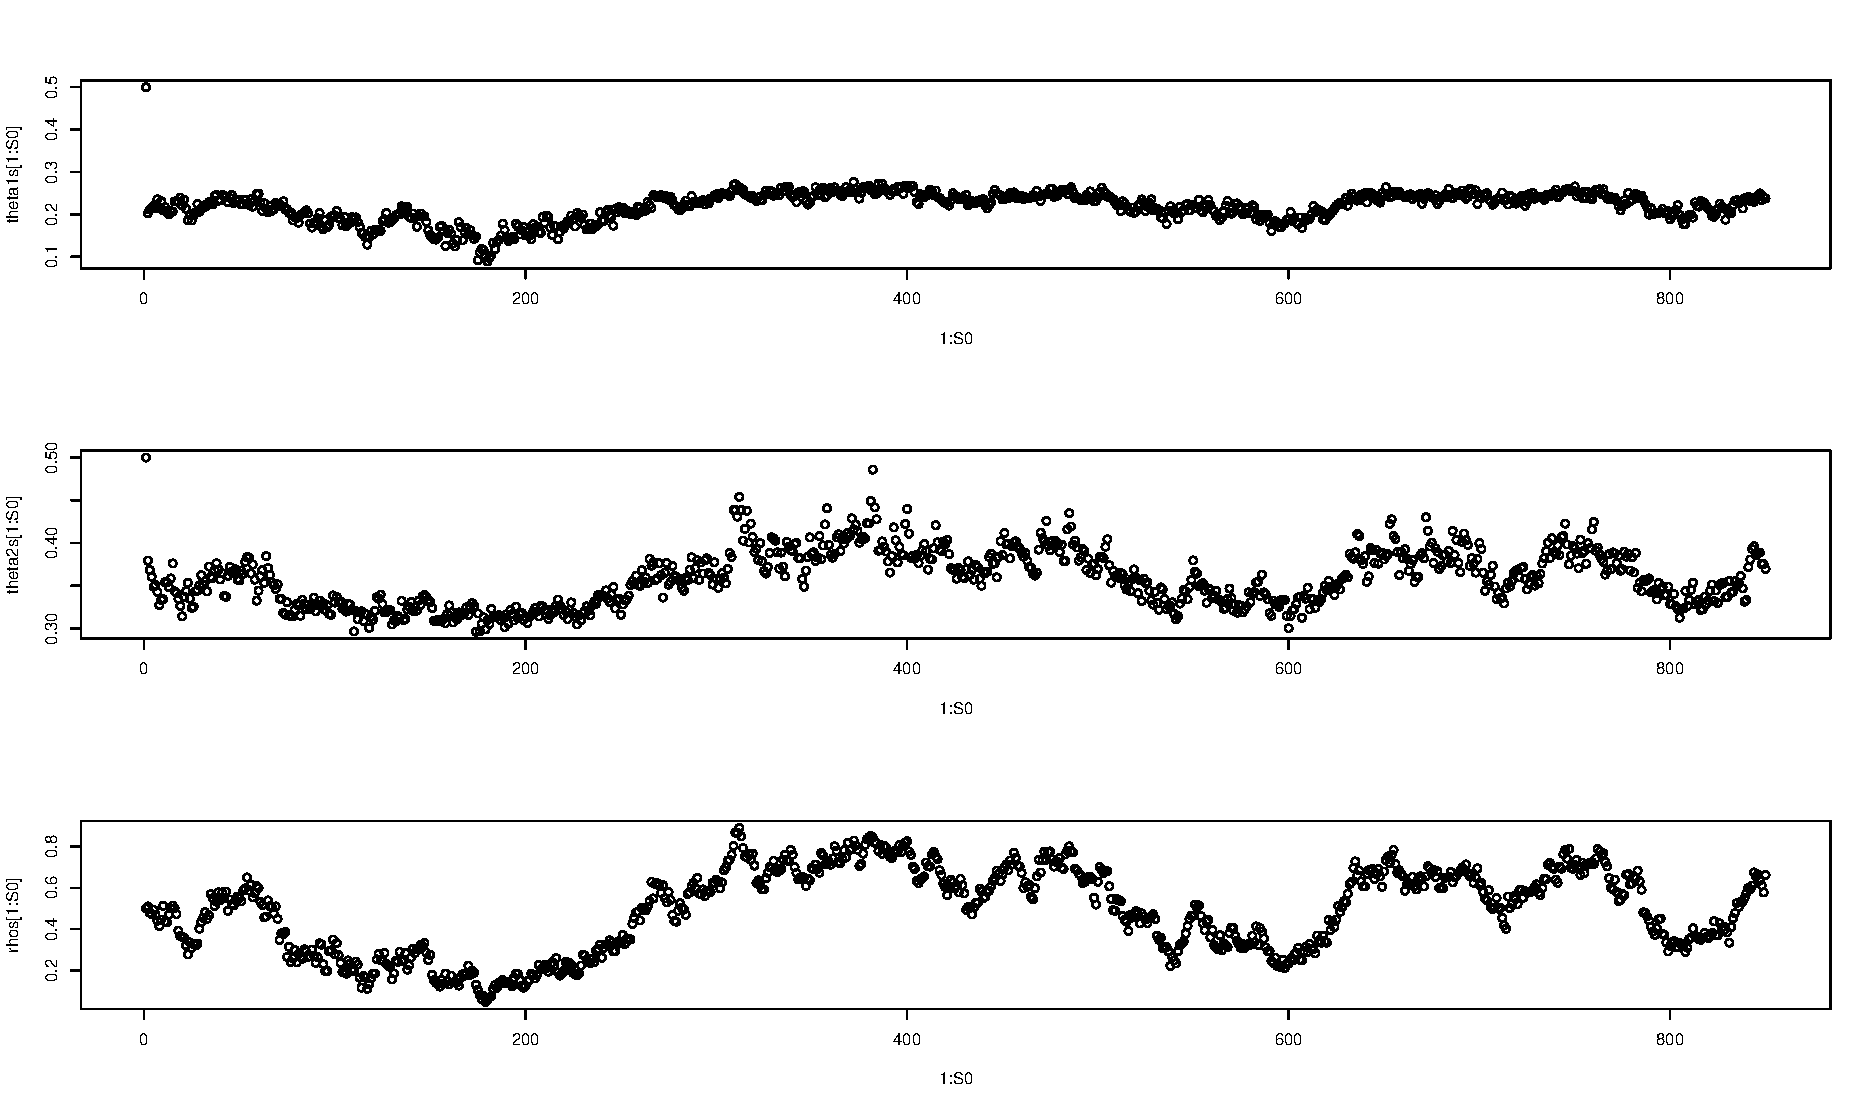
\includegraphics[width=7in]{burn}
\end{figure}

\benum\subquestionwithpoints{4} Where should we burn-in the chain? Select the best answer below:

\begin{enumerate}[(a)]
\item 10
\item 380
\item 750
\item never
\end{enumerate}\eenum\instr\pagebreak
%%%%%%%%%%%%%%%%%%%%%%%%


\problem [4min] \ingray{We employ the Gibbs sampler specified previously to provide $\iid$ samples from the posterior $\cprob{\theta_L, \theta_R, \rho, I_1, \ldots, I_G}{X}$. We run $S=100,000$ samples.} We appropriately burned in. Now we wish to thin the chain. Below are autocorrelation plots. The top plot is the chain for $\theta_L~|~X$, the middle plot is the chain for $\theta_R~|~X$ and the bottom plot is the chain for $\rho~|~X$. The chains for $I_1~|~X, \ldots, I_G~|~X$ are not displayed.

\begin{figure}[h]
\centering
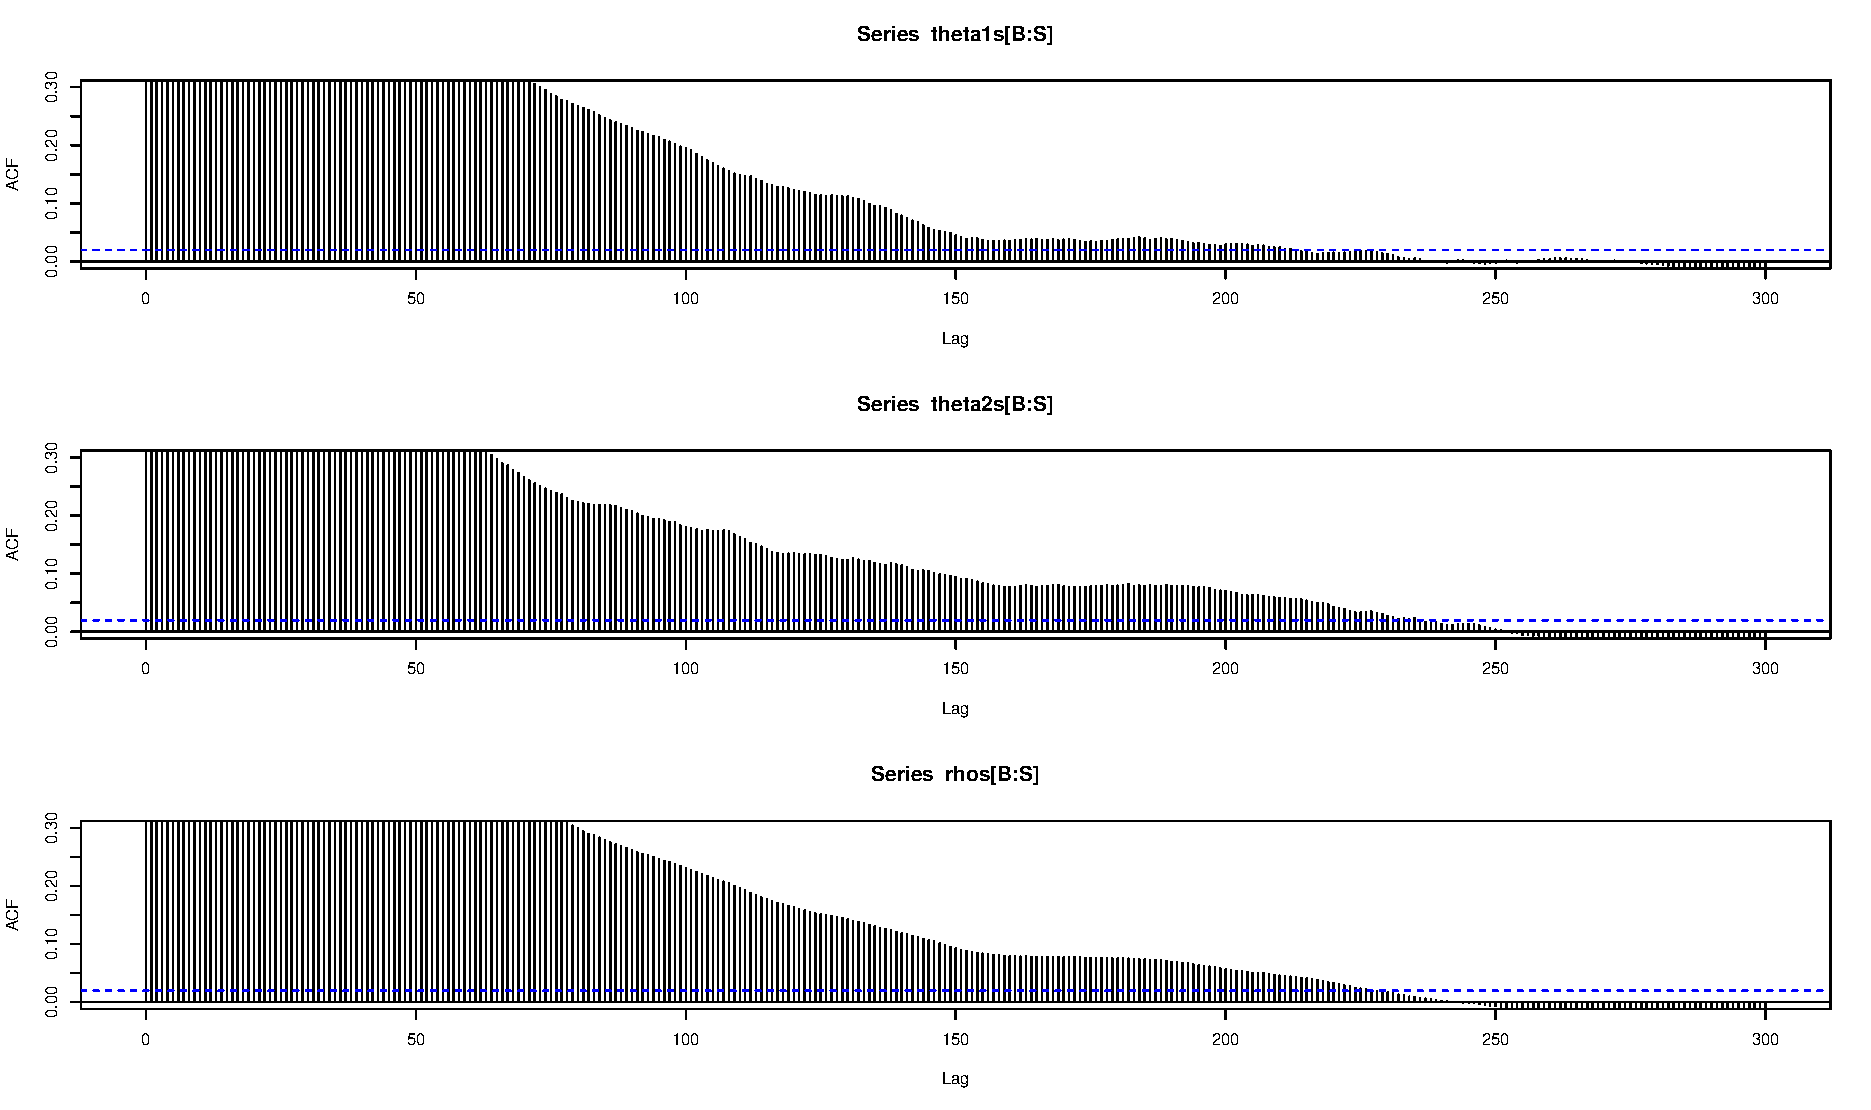
\includegraphics[width=7in]{thin}
\end{figure}

\benum\subquestionwithpoints{4} What multiple of the chain samples should we thin? Select the best answer below:

\begin{enumerate}[(a)]
\item 10
\item 100
\item 250
\item never
\end{enumerate}\eenum\instr\pagebreak


\problem [6min] \ingray{We employ the Gibbs sampler specified previously to provide $\iid$ samples from the posterior $\cprob{\theta_L, \theta_R, \rho, I_1, \ldots, I_G}{X}$. We run $S=100,000$ samples.} We appropriately burned and thinned and now we provide histograms for the marginal posteriors.  Below is a plot for $\theta_L$.

\begin{figure}[h]
\centering
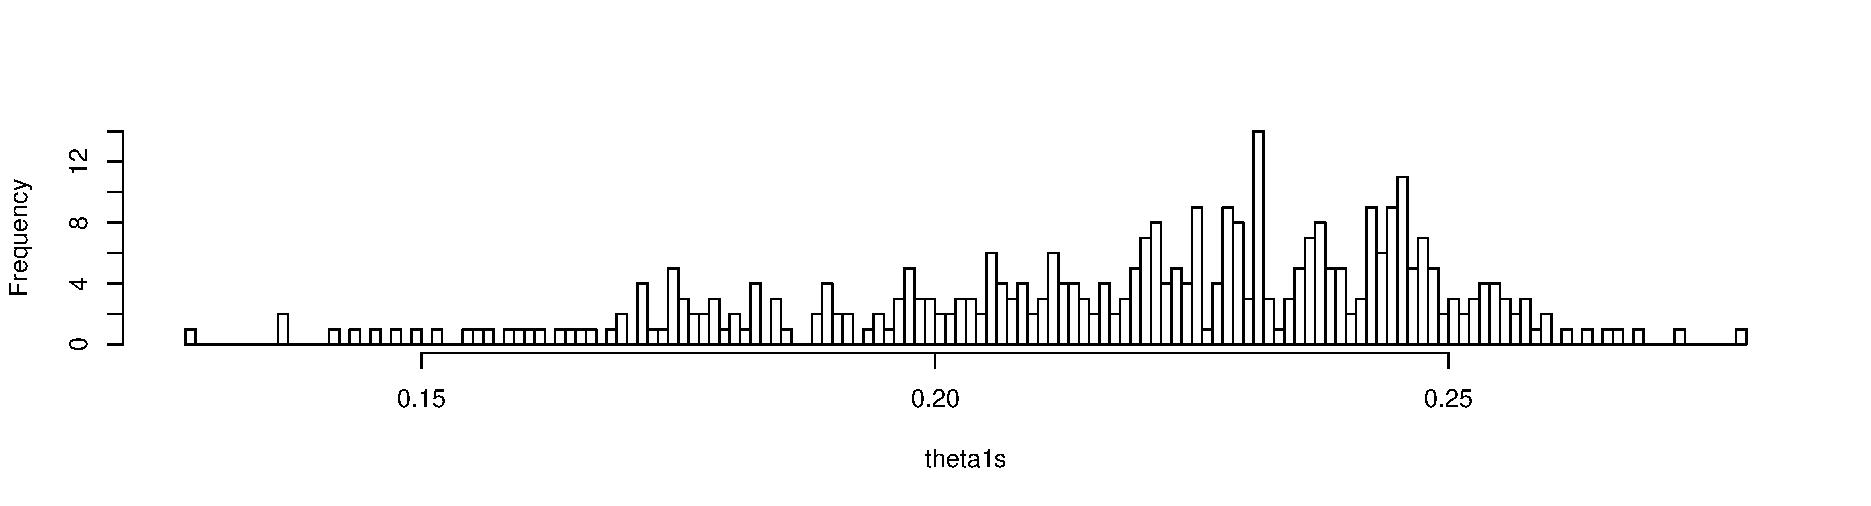
\includegraphics[width=7in]{theta1s}
\end{figure}

\vspace{-1cm}
\benum\subquestionwithpoints{12} \recordletters

\begin{enumerate}[(a)]
\item The above approximates $\cprob{\theta_L}{X, \theta_R, \rho, I_1, \ldots, I_G}$ 
\item The above approximates $\cprob{\theta_L}{X, \theta_R, \rho}$ 
\item The above approximates $\cprob{\theta_L}{X}$ 
\item The MMSE for $\theta_L$ is approximately 0.15
\item The MMSE for $\theta_L$ is approximately 0.20
\item The MMSE for $\theta_L$ is approximately 0.22
\item The MMSE for $\theta_L$ is equal to the MMAE for $\theta_L$.
\item The MMSE for $\theta_L$ is larger than the MMAE for $\theta_L$.
\item A 95\% credible region for $\theta_L$ is impossible to estimate from this plot alone.
\item This plot alone will allow us to test if $\theta_L \neq \theta_R$.
\item If you are testing if $\theta_L > 0.15$, the p value would be small and the null likely rejected.
\end{enumerate}\eenum\instr\pagebreak
%%%%%%%%%%%%%%%%%%%%%%%%


\problem [6min] \ingray{We employ the Gibbs sampler specified previously to provide $\iid$ samples from the posterior $\cprob{\theta_L, \theta_R, \rho, I_1, \ldots, I_G}{X}$. We run $S=100,000$ samples. We appropriately burned and thinned and now we provide histograms for the marginal posteriors.} Below is a plot for $\rho$.

\begin{figure}[h]
\centering
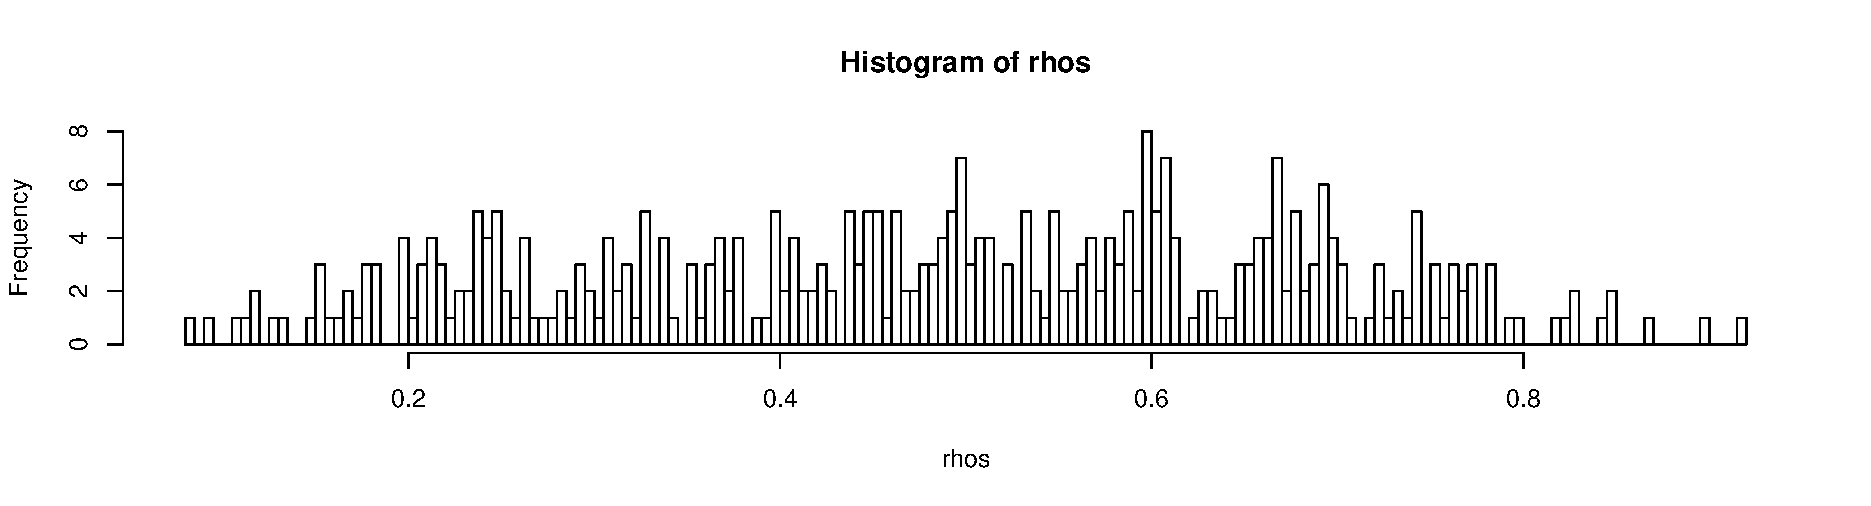
\includegraphics[width=7in]{rhos}
\end{figure}

\vspace{-1cm}
\benum\subquestionwithpoints{5} \recordletters

\begin{enumerate}[(a)]
\item The above approximates $\cprob{\rho}{X}$ 
\item A 95\% credible region for $\rho$ would range from 0.1 to 0.9.
\item The main conclusion here is that $\rho$ cannot be estimated well.
\item The MMSE for $\rho$ is nearly equal to the MMAE for $\rho$.
\item Based on the plot above, estimates for most of the $I_i$'s will be ambiguous.
\end{enumerate}\eenum\instr\pagebreak
%%%%%%%%%%%%%%%%%%%%%%%%


\problem [10min] \ingray{We employ the Gibbs sampler specified previously to provide $\iid$ samples from the posterior $\cprob{\theta_L, \theta_R, \rho, I_1, \ldots, I_G}{X}$. We run $S=100,000$ samples. We appropriately burned and thinned and now we provide histograms for the marginal posteriors.}  Below is a plot for each $\theta_L$ sample subtracted from each $\theta_R$ sample.

\begin{figure}[h]
\centering
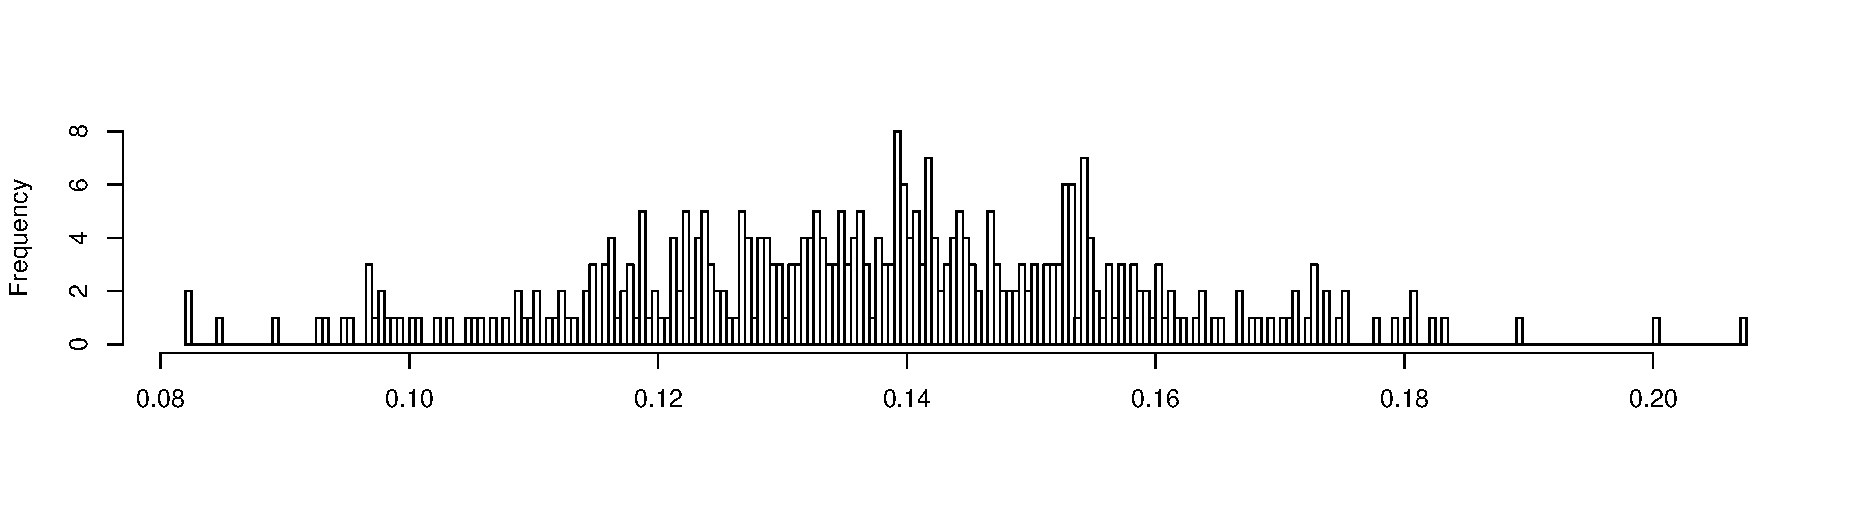
\includegraphics[width=7in]{thetaLminusthetaRs}
\end{figure}

\vspace{-1cm}
\benum\subquestionwithpoints{10} \recordletters

\begin{enumerate}[(a)]
\item The above plot approximates $\cprob{\theta_R - \theta_L}{X}$.
\item The above plot tells us that more likely than not $\rho < 50\%$.
\item The main conclusion here is that $\rho$ cannot be estimated well.
\item This plot alone will allow us to test if $\theta_R \neq \theta_L$.
\item The null hypothesis that $\theta_R = \theta_L$ will result in a p-value estimated to be $\approx 0$.
\item The null hypothesis that $\theta_R = \theta_L$ will result in a p-value estimated to be $= 0$.
\item One can conclude from this plot that this batter is better at batting rightie than leftie.
\item One can conclude from this plot that this batter has about a 14\% higher probability of getting a hit when batting rightie than leftie.\\

The $I_1$ distribution after burning and thinning is 14 0's and 343 1's.

\item The probability that the batter bat leftie for game \#1 is about 96\%.
\item The best guess as to his batting orientation for game \#1 is leftie.
\end{enumerate}\eenum\instr\pagebreak
%%%%%%%%%%%%%%%%%%%%%%%%


\problem [4min] \ingray{ Imagine the batter bats both leftie and rightie (both sides of the oncoming ball). The propensity to get a hit when batting leftie is $\theta_L$ and the propensity to get a hit on when batting rightie is $\theta_R$. He bats leftie $\rho$ proportion of the games. Let $I_i$ be the indicator variable indicating if he bats leftie for the $i$th game (it is equal to 1 when he bats leftie and equal to 0 if he bats rightie). There are $n$ independent at bats per game and $G$ independent total games per season and both $n$ and $G$ are known. The data $x_1, \ldots, x_G$ are number of hits per game. All other quantities are unknown.  All sum signs are indexed from $1, \ldots, G$.} Here is a histogram of the original data for the $G = 300$ games:

\begin{figure}[h]
\centering
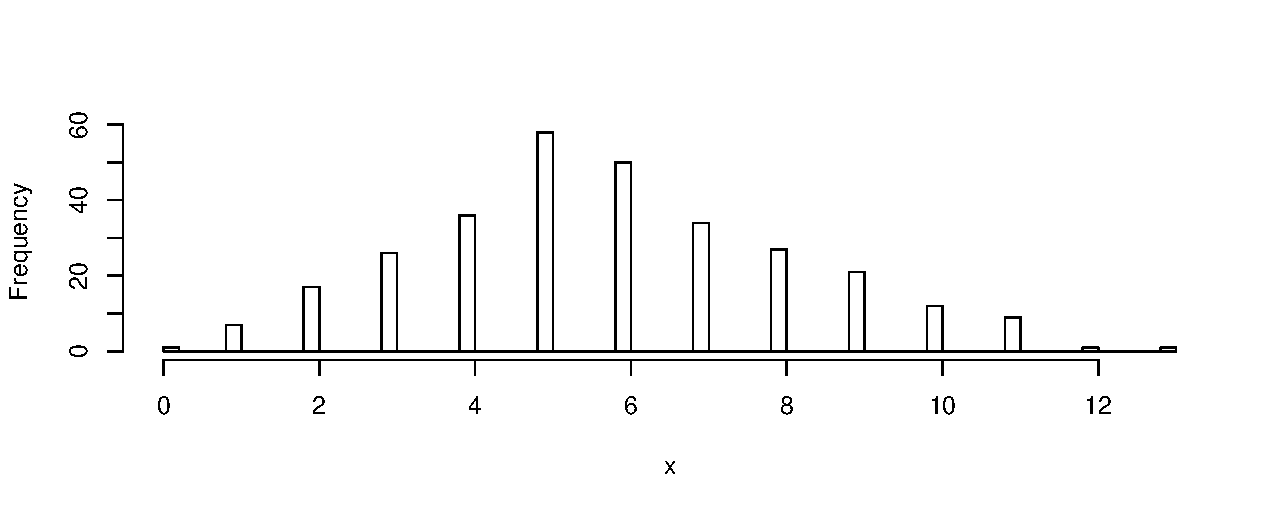
\includegraphics[width=7in]{xs}
\end{figure}

\vspace{-1cm}
\benum\subquestionwithpoints{10} \recordletters

\begin{enumerate}[(a)]
\item This data indicates that our model formulation $\mathcal{F}$ must be incorrect.
\item This data indicates that a betabinomial model may be appropriate.
\item If the model is correctly formulated, this data shows that $\theta_L$ and $\theta_R$ are similar.
\item If the model is correctly formulated, this data shows that $\rho$ is difficult to estimate.
\item If the model is correctly formulated, this data shows that the $I_i$'s are difficult to estimate.
\end{enumerate}\eenum\instr\pagebreak
%%%%%%%%%%%%%%%%%%%%%%%%


\problem [17min] Let $\mathcal{F}: \iid \normnot{\theta}{\sigsq}$ with both $\theta$ and $\sigsq$ unknown.


\benum\subquestionwithpoints{20} \recordletters

\begin{enumerate}[(a)]
\item The prior $\prob{\theta, \sigsq}$ being normal is conjugate to the posterior which is normal.
\item The prior $\prob{\theta, \sigsq}$ being normal-inverse-gamma is conjugate to the posterior which is normal.
\item The prior $\prob{\theta, \sigsq}$ being normal-inverse-gamma is conjugate to the posterior which is normal-inverse-gamma.
\item The prior $\prob{\theta, \sigsq} \propto 1$ is conjugate.
\item The prior $\prob{\theta, \sigsq} \propto 1/{\sigsq}$ is conjugate.
\item The prior $\cprob{\theta}{\sigsq}\prob{\sigsq}$ is always conjugate.
\item The prior $\prob{\theta}\prob{\sigsq}$ is always semi-conjugate.
\item The prior $\cprob{\theta}{\sigsq}\prob{\sigsq}$ is conjugate only if $\cprob{\theta}{\sigsq} = \normnot{\mu_0}{\sigsq / n_0}$ and $\prob{\sigsq}$ is inverse gamma.
\item The prior $\cprob{\theta}{\sigsq}\prob{\sigsq}$ is conjugate only if $\cprob{\theta}{\sigsq} = \normnot{\mu_0}{\tausq}$ and $\prob{\sigsq}$ is inverse gamma where $\tausq$ is a constant.
\item A conjugate prior will yield a posterior kernel $k(\theta, \sigsq\,|\,X) = \tothepow{\sigsq}{-\alpha - 1} e^{-(\beta + \lambda \squared{\theta - \mu_0}) / \sigsq}$ where $\alpha, \beta, \lambda, \mu_0$ are constants which do not depend on $\theta$ or $\sigsq$. \\

Regardless of whether (j) was true, assume this kernel for the rest of the problem.

\item If $k(\theta, \sigsq\,|\,X)$ is factored into $k(\theta|\,X, \sigsq) k(\sigsq\,|\,X)$ then $k(\theta|\,X, \sigsq) \propto$ a normal.
\item If $k(\theta, \sigsq\,|\,X)$ is factored into $k(\theta|\,X, \sigsq) k(\sigsq\,|\,X)$ then $k(\theta|\,X, \sigsq)$ is a kernel for no known random variable.
\item If $k(\theta, \sigsq\,|\,X)$ is factored into $k(\theta|\,X, \sigsq) k(\sigsq\,|\,X)$ then $k(\sigsq|\,X) \propto$ an inverse gamma distribution.
\item If $k(\theta, \sigsq\,|\,X)$ is factored into $k(\theta|\,X, \sigsq) k(\sigsq\,|\,X)$ then $k(\sigsq|\,X)$ is a kernel for no known random variable.
\item It can be shown that $\int_0^\infty k(\theta, \sigsq\,|\,X) d\sigsq \propto$ a normal distribution.
\item It can be shown that $\int_0^\infty k(\theta, \sigsq\,|\,X) d\sigsq \propto$ a students $T$ distribution.
\item It can be shown that $\int_0^\infty k(\theta, \sigsq\,|\,X) d\sigsq \propto$ an inverse gamma distribution.

\item It can be shown that $\int_\reals k(\theta, \sigsq\,|\,X) d\theta \propto$ a normal distribution.
\item It can be shown that $\int_\reals k(\theta, \sigsq\,|\,X) d\theta \propto$ a students $T$ distribution.
\item It can be shown that $\int_\reals k(\theta, \sigsq\,|\,X) d\theta \propto$ an inverse gamma distribution.
\end{enumerate}\eenum\instr\pagebreak
%%%%%%%%%%%%%%%%%%%%%%%%




\problem [7min] Let $\mathcal{F}: \iid \poisson{\theta}$. Let $\prob{\theta} = \gammanot{\alpha}{\beta}$,  $X_*$ represent the future observation(s) and $n_*$ represent the number of future observation(s).

\benum\subquestionwithpoints{12} \recordletters

\begin{enumerate}[(a)]
\item $\cprob{X}{\theta} = \cprob{X_1}{\theta} \cdot \cprob{X_2}{\theta} \cdot \ldots \cdot  \cprob{X_n}{\theta}$.
\item The prior is conjugate.
\item The prior is proper regardless of the values of $\alpha$ and $\beta$.
\item The posterior predictive distribution $\cprob{X_*}{X}$ is always negative binomial.
\item $\cprob{X_*}{X}$ is only negative binomial if $n_* = 1$.
\item $\cprob{X_*}{X}$ is only negative binomial if $n_* > 1$.\\

Assume $n_* = 10$ for the remainder of this problem.

\item To sample one $X_*$, we first need to draw $\theta_{\text{samp}}$, a sample from $\cprob{\theta}{X}$.
\item To sample one $X_*$, we first need to draw $\theta_{\text{samp}}$, a sample from $\prob{\theta}$.
\item To sample one $X_*$, we then draw $X_{\text{samp}, 1}, X_{\text{samp}, 2}, \ldots, X_{\text{samp}, n}$ values independently using \texttt{rpois}($\theta_{\text{samp}}$).
\item To sample one $X_*$, we then draw $X_{\text{samp}, 1}, X_{\text{samp}, 2}, \ldots, X_{\text{samp}, 10}$ values independently using \texttt{rpois}($\theta_{\text{samp}}$).
\item Regardless of the method used to sample one $X_*$, the components of $X_*$ are all independent of each other.
\item To sample many $X_*$'s, we repeat the procedure of correctly drawing $\theta_{\text{samp}}$ and then correctly drawing $X_*$ over and over again.
\end{enumerate}\eenum\instr\pagebreak
%%%%%%%%%%%%%%%%%%%%%%%%


\end{document}
